\documentclass{elegantbook}

\definecolor{LightGray}{gray}{0.9}
\newcommand{\CN}{BIOS 7300\\[0.5cm] Survival Data Analysis}
\newcommand{\Ti}{Homework 8}
\newcommand{\Pf}{Dr.\ Tang}
\newcommand{\FN}{Zehao}
\newcommand{\LN}{Wang}
\usepackage[fontsize=14pt]{fontsize}

\usepackage{longtable}

\usepackage{minted}

\usepackage{enumitem}
\renewcommand{\chaptername}{Homework}
\begin{document} 
\begin{titlepage}
    \begin{center}    
    
\includegraphics[width=0.6\textwidth]{Tulane.png}\\[1cm]    
    
    \textsc{\Huge \CN}\\[0.5cm]
    \textsc{\large \Pf}\\[1.0cm]
    
    \textsc{\LARGE \Ti}\\[0.5cm]
    \textsc{\large \LN, \FN}\\
    {Master student in Statistics of Math Dept.}
    
    % Author and supervisor
    
    \vfill
    
    % Bottom of the page
    {\Large \emph{\today}}
    
    \end{center}
\end{titlepage}

\thispagestyle{empty}
\tableofcontents
\setcounter{chapter}{7}
\chapter{}
\begin{exercise*}[1]
    In the Worcester Heart Attack Study (file “whas500.sas7bdat”), we are interested in the survival time since the hospital admission. “LENFOL” is total length of follow-up and FSTAT is the status at the last follow-up (0 = alive, hence censoring, and 1 = death). Consider the following Cox proportional hazards model: 
    \begin{center}
        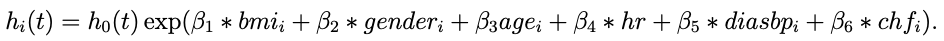
\includegraphics[width=.95\textwidth]{Q1.png}
    \end{center}
    We will assess this model through residual analysis, influential analysis, and testing the proportional hazards assumption. 
    \begin{enumerate}
        \item By looking at the residuals, we may identify potential outliers and potential problems of the model.
        \begin{enumerate}[(a)]
            \item Compute the martingale, deviance, and scaled Schoenfeld residuals and identify subjects with the five largest and five lowest (largest negative) values in each of the residuals.
            \item Plot the cumulative hazard plot of the Cox-Snell residuals to assess the model. Does this plot suggest any problem of the model?
            \item Plot the martingale and deviance residuals vs the rank order of the survival times. Do these plots suggest any problem of the model?
            \item Let us assume that the functional form for the other covariates are correct, and we want to assess the functional form of bmi. Plot the martingale residual of the model without bmi as a covariate vs the bmi values and fit it with a smooth curve. Will the plot confirm a linear relationship for bmi?
        \end{enumerate}
        \item Influential analysis. 
        \begin{enumerate}[(a)]
            \item Identify five subjects with the largest impact on the overall fit of the model (LD and LMAX).
            \item Identify five subjects with the largest impact on the coefficient of bmi, β1, using the approximation dfbeta.
            \item If the subject with highest impact on β1 is deleted, how much is actual change in the estimation of β1? 
        \end{enumerate}
        \item Assessing the proportional hazards hypothesis. 
        \begin{enumerate}[(a)]
            \item Dichotomizing the subjects according to bmi $\leq25$ and $> 25$, and plot the log-cumulative hazard vs log of survival time to check the  proportional hazards assumption between the two groups. 
            \item We can formally test the assumption by testing whether the coefficients, $\beta_i$, are time varying. Test whether $\beta_1$, the coefficient of bmi, is time varying by assuming $\beta_1(t)=\beta_1+\gamma_1\log(t)$. 
            \item Perform a global testing of whether all the coefficients are time varying (use $g(t)=\log t$ for all the coefficient).
        \end{enumerate}
    \end{enumerate}
\end{exercise*}

\begin{solution}
    \begin{enumerate}
        \item 
        \begin{enumerate}[(a)]
            \item \begin{minted}[frame=lines,
                framesep=2mm,
                baselinestretch=1.2,
                bgcolor=LightGray,
                fontsize=\footnotesize]{SAS}
DATA HW8;
SET "Z:\Documents\GitHub\MS-Stat-Tulane
\Survival Data Analysis\HW08\whas500.sas7bdat";
PROC PHREG DATA = HW8; 
CLASS GENDER CHF; 
MODEL LENFOL*FSTAT(0) = BMI GENDER AGE HR DIASBP CHF; 
OUTPUT OUT = a LOGSURV=LOGSURV RESDEV=RESDEV RESMART =RESMART
WTRESSCH = WRESSCH1 WRESSCH2 WRESSCH3 WRESSCH4 WRESSCH5 WRESSCH6
/METHOD = ch;
PROC UNIVARIATE DATA = a; 
VAR RESDEV RESMART WRESSCH1 WRESSCH2 WRESSCH3 
    WRESSCH4 WRESSCH5 WRESSCH6; 
RUN; 
            \end{minted}
            Deviance: \begin{center}
                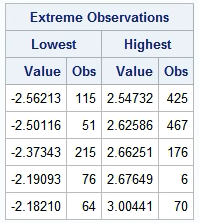
\includegraphics[width=.3\textwidth]{dev.png}
            \end{center}
            Martingale: \begin{center}
                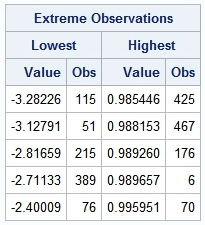
\includegraphics[width=.3\textwidth]{mar.png}
            \end{center}
            Standardized Schoenfeld Residual BMI: \begin{center}
                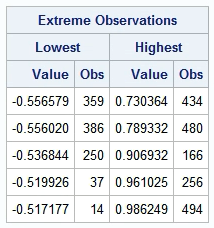
\includegraphics[width=.3\textwidth]{bmi.png}
            \end{center}
            Standardized Schoenfeld Residual GENDER0: \begin{center}
                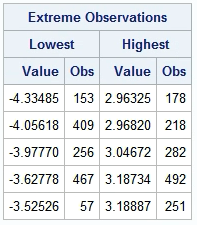
\includegraphics[width=.3\textwidth]{gender0.png}
            \end{center}
            Standardized Schoenfeld Residual AGE: \begin{center}
                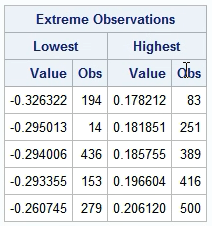
\includegraphics[width=.3\textwidth]{age.png}
            \end{center}
            Standardized Schoenfeld Residual HR: \begin{center}
                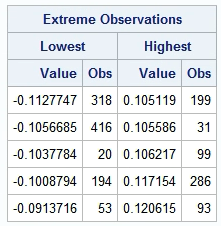
\includegraphics[width=.3\textwidth]{hr.png}
            \end{center}
            Standardized Schoenfeld Residual DIASBP: \begin{center}
                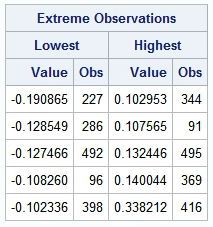
\includegraphics[width=.3\textwidth]{diasbp.png}
            \end{center}
            Standardized Schoenfeld Residual CHF0: 
            \begin{center}
                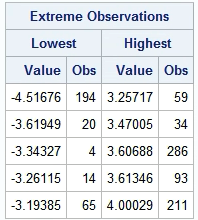
\includegraphics[width=.3\textwidth]{chf0.png}
            \end{center}
            \item \begin{minted}[frame=lines,
                framesep=2mm,
                baselinestretch=1.2,
                bgcolor=LightGray,
                fontsize=\footnotesize]{SAS}
DATA a;
SET a;
r = -logsurv;
PROC LIFETEST data = a plot = LOGSURV;
TIME r*FSTAT(0);
SURVIVAL OUT = b ;
RUN;
            \end{minted}
            \begin{center}
                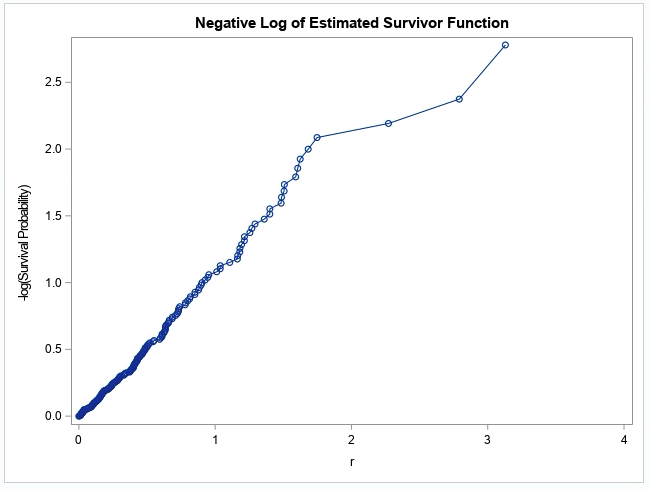
\includegraphics[width=.7\textwidth]{q1b.png}
            \end{center}
            Most of the points are in a straight line, which suggests that the model is good. 
            \item \begin{minted}[frame=lines,
                framesep=2mm,
                baselinestretch=1.2,
                bgcolor=LightGray,
                fontsize=\footnotesize]{SAS}
PROC RANK DATA = a TIES = mean OUT = b ;
VAR LENFOL; RANKS LENFOLRANK; 
PROC SGPLOT DATA = b;
YAXIS GRID; 
REFLINE 0 / AXIS = y; 
SCATTER Y = RESDEV X = LENFOLRANK;
RUN; 
PROC SGPLOT DATA = b;
YAXIS GRID; 
REFLINE 0 / AXIS = y; 
SCATTER Y = RESMART X = LENFOLRANK;
RUN; 
            \end{minted}
            \begin{center}
                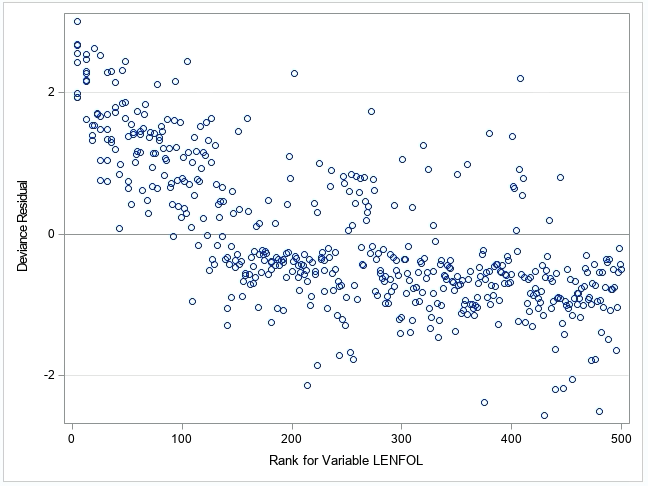
\includegraphics[width=.4\textwidth]{q1c1.png}
                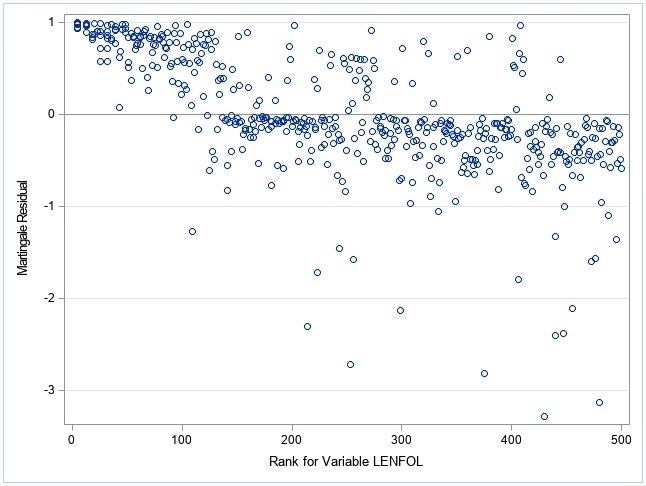
\includegraphics[width=.4\textwidth]{q1c2.png}
            \end{center}
            From these two plots, we can see that there is no outliers. 
            \item \begin{minted}[frame=lines,
                framesep=2mm,
                baselinestretch=1.2,
                bgcolor=LightGray,
                fontsize=\footnotesize]{SAS}
PROC PHREG DATA = HW8; 
CLASS GENDER CHF; 
MODEL LENFOL*FSTAT(0) = GENDER AGE HR DIASBP CHF; 
OUTPUT OUT = a RESMART = RESMART;
DATA a;
SET a;
logbmi = log(BMI);
PROC LOESS DATA = a;
MODEL RESMART = logbmi;
RUN;
            \end{minted}
            \begin{center}
                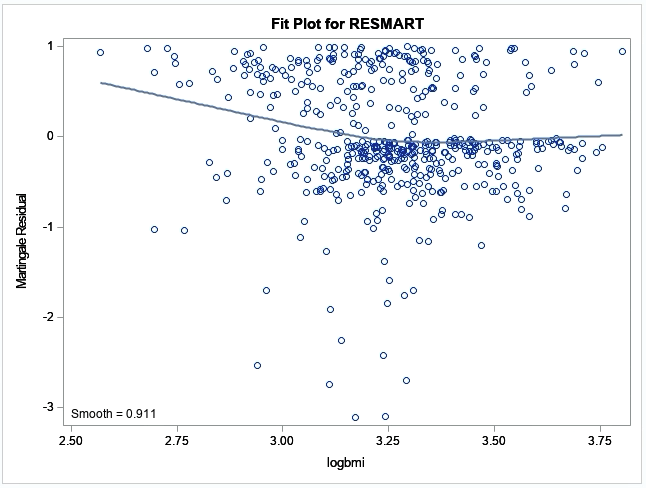
\includegraphics[width=.7\textwidth]{q1d.png}
            \end{center}
            We could see that smooth is 0.911, that means there is a linear relationship for bmi. 
        \end{enumerate}
        \item \begin{enumerate}[(a)]
            \item \begin{minted}[
                frame=lines,
                framesep=2mm,
                baselinestretch=1.2,
                bgcolor=LightGray,
                fontsize=\footnotesize]{SAS}
PROC PHREG DATA = HW8; 
CLASS GENDER CHF; 
MODEL LENFOL*FSTAT(0) = BMI GENDER AGE HR DIASBP CHF; 
OUTPUT OUT = a LOGSURV = LOGSURV LMAX = LMAX 
    LD = LD DFBETA = DBMI/METHOD = ch;
PROC UNIVARIATE DATA = a; 
VAR LMAX LD DBMI; 
RUN; 
            \end{minted}
            \begin{center}
                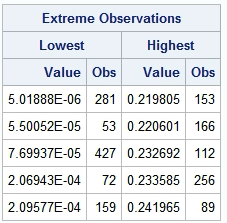
\includegraphics[width=.3\textwidth]{q2a1.png}
                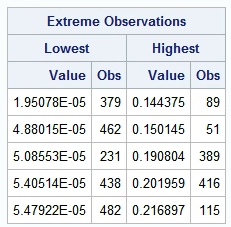
\includegraphics[width=.305\textwidth]{q2a2.png}
            \end{center}
            LMAX: 153, 166, 112, 256, 89; 

            LD: 89, 51, 389, 416, 115. 
            \item For $\beta_1$, Five largest impact subjects are: 112, 494, 166, 256, 115. 
            \begin{center}
                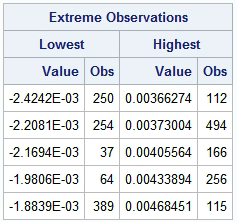
\includegraphics[width=.3\textwidth]{q2b.png}
            \end{center}
            \item \begin{minted}[
                frame=lines,
                framesep=2mm,
                baselinestretch=1.2,
                bgcolor=LightGray,
                fontsize=\footnotesize]{SAS}
PROC PHREG DATA = HW8; 
CLASS GENDER CHF; 
MODEL LENFOL*FSTAT(0) = BMI GENDER AGE HR DIASBP CHF; 
RUN; 
DATA HW8_1;
SET HW8;
IF ID = "115" THEN DELETE;
PROC PHREG DATA = HW8_1;
CLASS GENDER CHF; 
MODEL LENFOL*FSTAT(0) = BMI GENDER AGE HR DIASBP CHF; 
RUN;         
            \end{minted}
            The actual change is $-0.04516+0.05029=0.00513$. 
            \begin{center}
                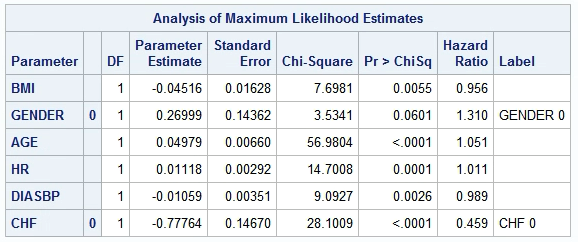
\includegraphics[width=.6\textwidth]{q2c1.png}
                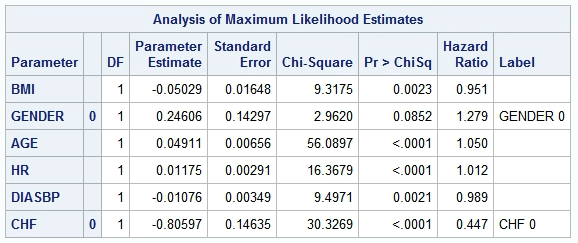
\includegraphics[width=.6\textwidth]{q2c2.png}
            \end{center}
        \end{enumerate}
        \item \begin{enumerate}[(a)]
            \item \begin{minted}[frame=lines,
                framesep=2mm,
                baselinestretch=1.2,
                bgcolor=LightGray,
                fontsize=\footnotesize]{SAS}
DATA HW8_2; SET HW8;
IF BMI <= 25 THEN Group = 0;
IF BMI > 25 THEN Group = 1;
PROC LIFETEST DATA=HW8_2 METHOD=km PLOT = LLS;
TIME LENFOL*FSTAT(0);
STRATA Group;
RUN;
            \end{minted}
            We could see that these two lines are generally parallel, which the proportional hazards assumption is fine. 
            \begin{center}
                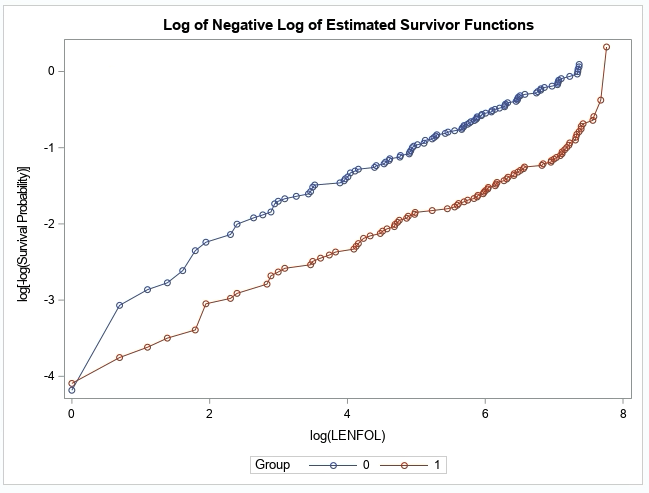
\includegraphics[width=.6\textwidth]{q3a.png}
            \end{center}
            \item \begin{minted}[frame=lines,
                framesep=2mm,
                baselinestretch=1.2,
                bgcolor=LightGray,
                fontsize=\footnotesize]{SAS}
PROC PHREG DATA = HW8 zph (global TRANSFORM=log);
CLASS GENDER CHF; 
MODEL LENFOL*FSTAT(0) = BMI GENDER AGE HR DIASBP CHF;
RUN;
            \end{minted}
            From the results, we can see that $p$-$value=0.2123>0.05$, which means $\beta_1$ is not time varying. 
            \begin{center}
                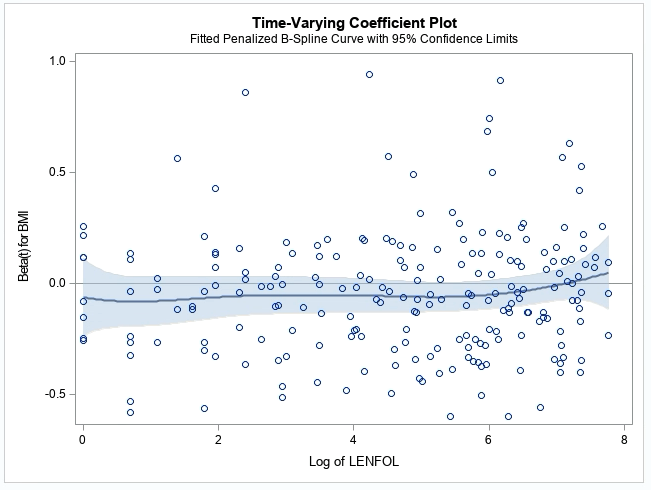
\includegraphics[width=.6\textwidth]{q3b1.png}
                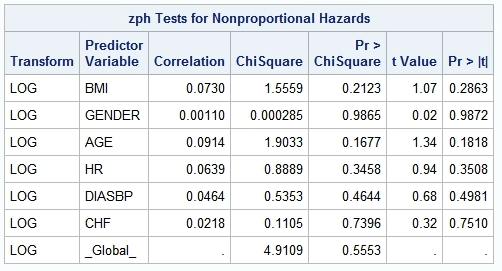
\includegraphics[width=.6\textwidth]{q3b2.png}
            \end{center}
            \item $p$-$value$ for Global tets is $0.5553>0.05$, i.e., all the coefficients are not time varying. 
        \end{enumerate}
    \end{enumerate}
\end{solution}
\end{document}